\documentclass[a4paper, 11pt]{article}
\usepackage{lipsum} %This package just generates Lorem Ipsum filler text. 
\usepackage{fullpage} % changes the margin
\usepackage{mathpazo}
\usepackage{multicol}
\usepackage{graphicx}
\usepackage{enumerate}
\usepackage{amsmath,amsfonts,amsthm} % Math packages
\usepackage{CJK}
\usepackage{listings}

\begin{document}
%Header-Make sure you update this information!!!!
\noindent
\large\textbf{Homework x} \hfill \textbf{Hongyu Yan (516030910595)} \\
\normalsize {\bf CS 259 Numerical Methods for Data Science} \hfill ACM Class, Zhiyuan College, SJTU\\
Prof.~{\bf David Bindel} \hfill Due Date: June 20, 2018\\
TA.~{\bf Yurong You, Xinran Zhu} \hfill Submit Date: \today

\section*{Problem 1}

The lagrangian $f(x)$ is 
$$f(x)=X^TMX + \lambda^T(AX-b)$$
So the KKT conditions are
\begin{align}
\nabla f(x) = 2MX + A^T\lambda &= 0 \\
AX-b &=0
\end{align}
From equation(1) we get 
\begin{align}
X = -\frac{1}{2}M^{-1}A^T\lambda
\end{align}
Substituting the equation(3) into the equation (2) gives:
\begin{align}
\frac{1}{2}AM^{-1}A^T\lambda=b
\end{align}
From the equation(4) we get
\begin{align}
\lambda = 2bA^{-T}MA^{-1}
\end{align}
Substitute it to the equation(3) then get X.

\section*{Problem 2}
Sometimes the curve become extremely strange (like figure1)

Test error: 4.335756e+04

After using Tikhonov inverse, Test error: 7.594892e+00

After using trucated SVD, Test error: 7.715455e+00

\begin{figure}[htbp]
\centering
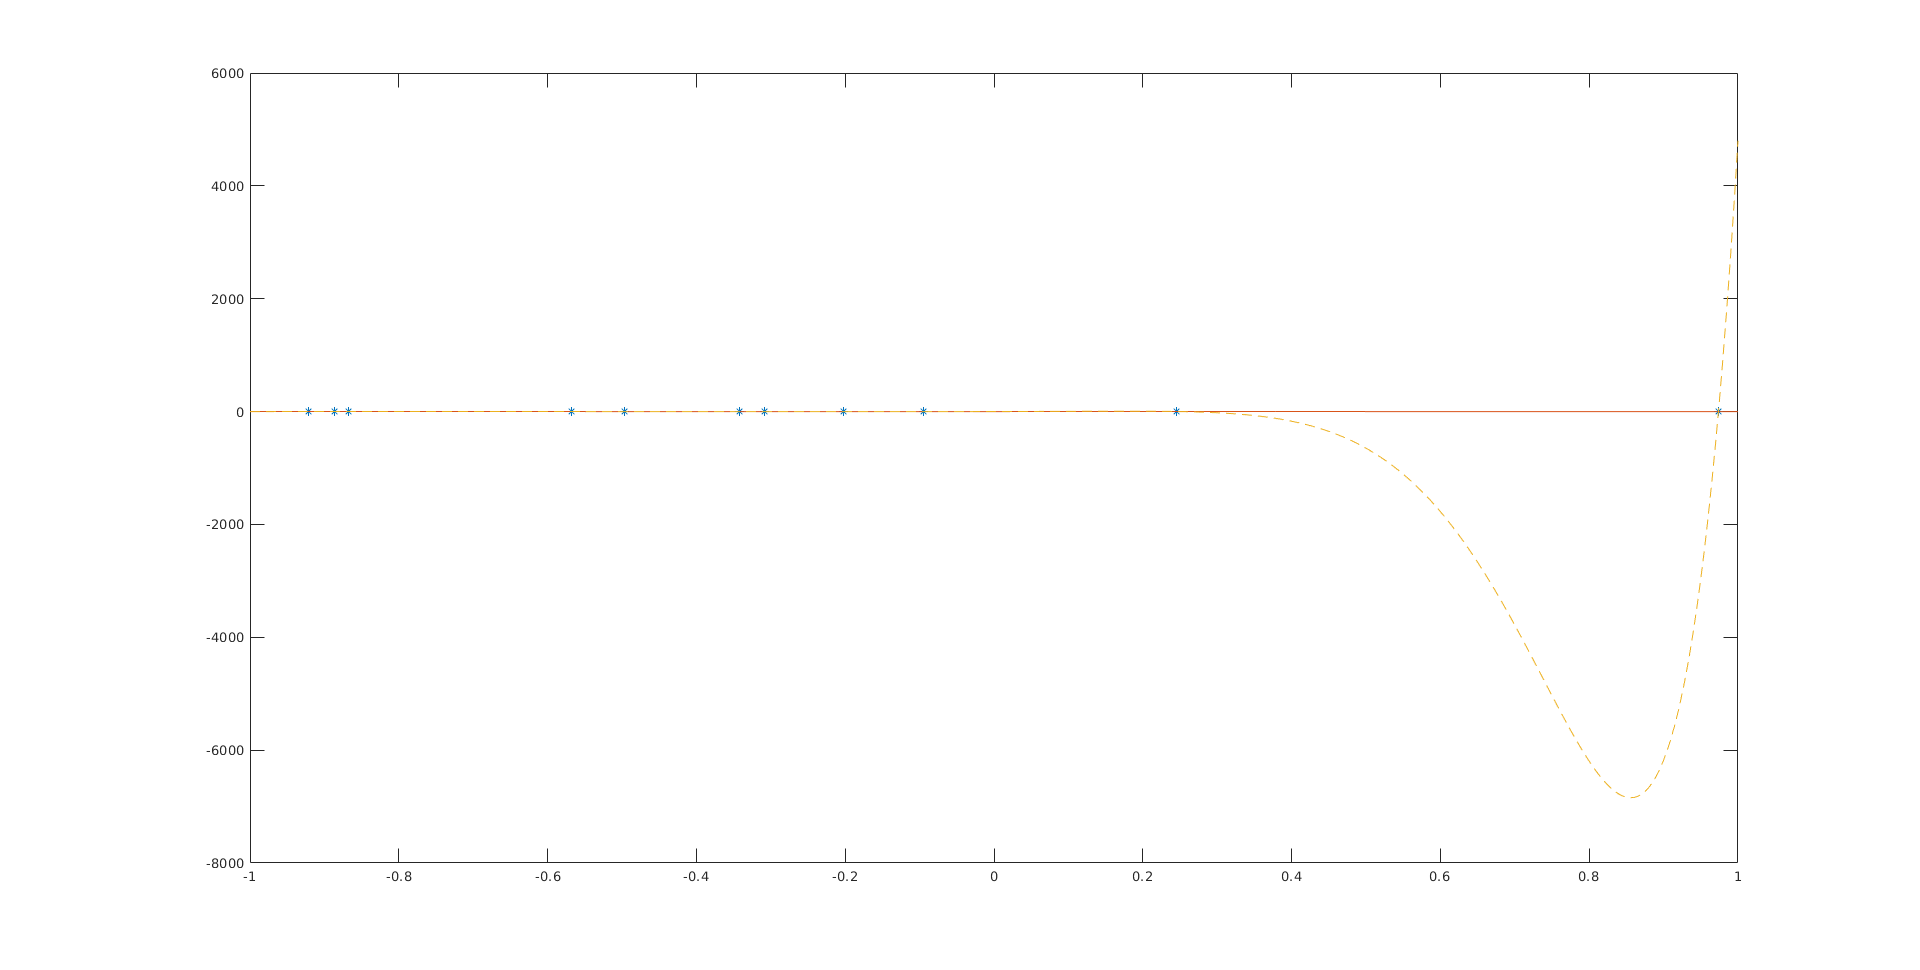
\includegraphics[scale=0.3]{figure/fig1.png}
\caption{original method}
\label{fig1}
\end{figure}

\begin{figure}[htbp]
\centering
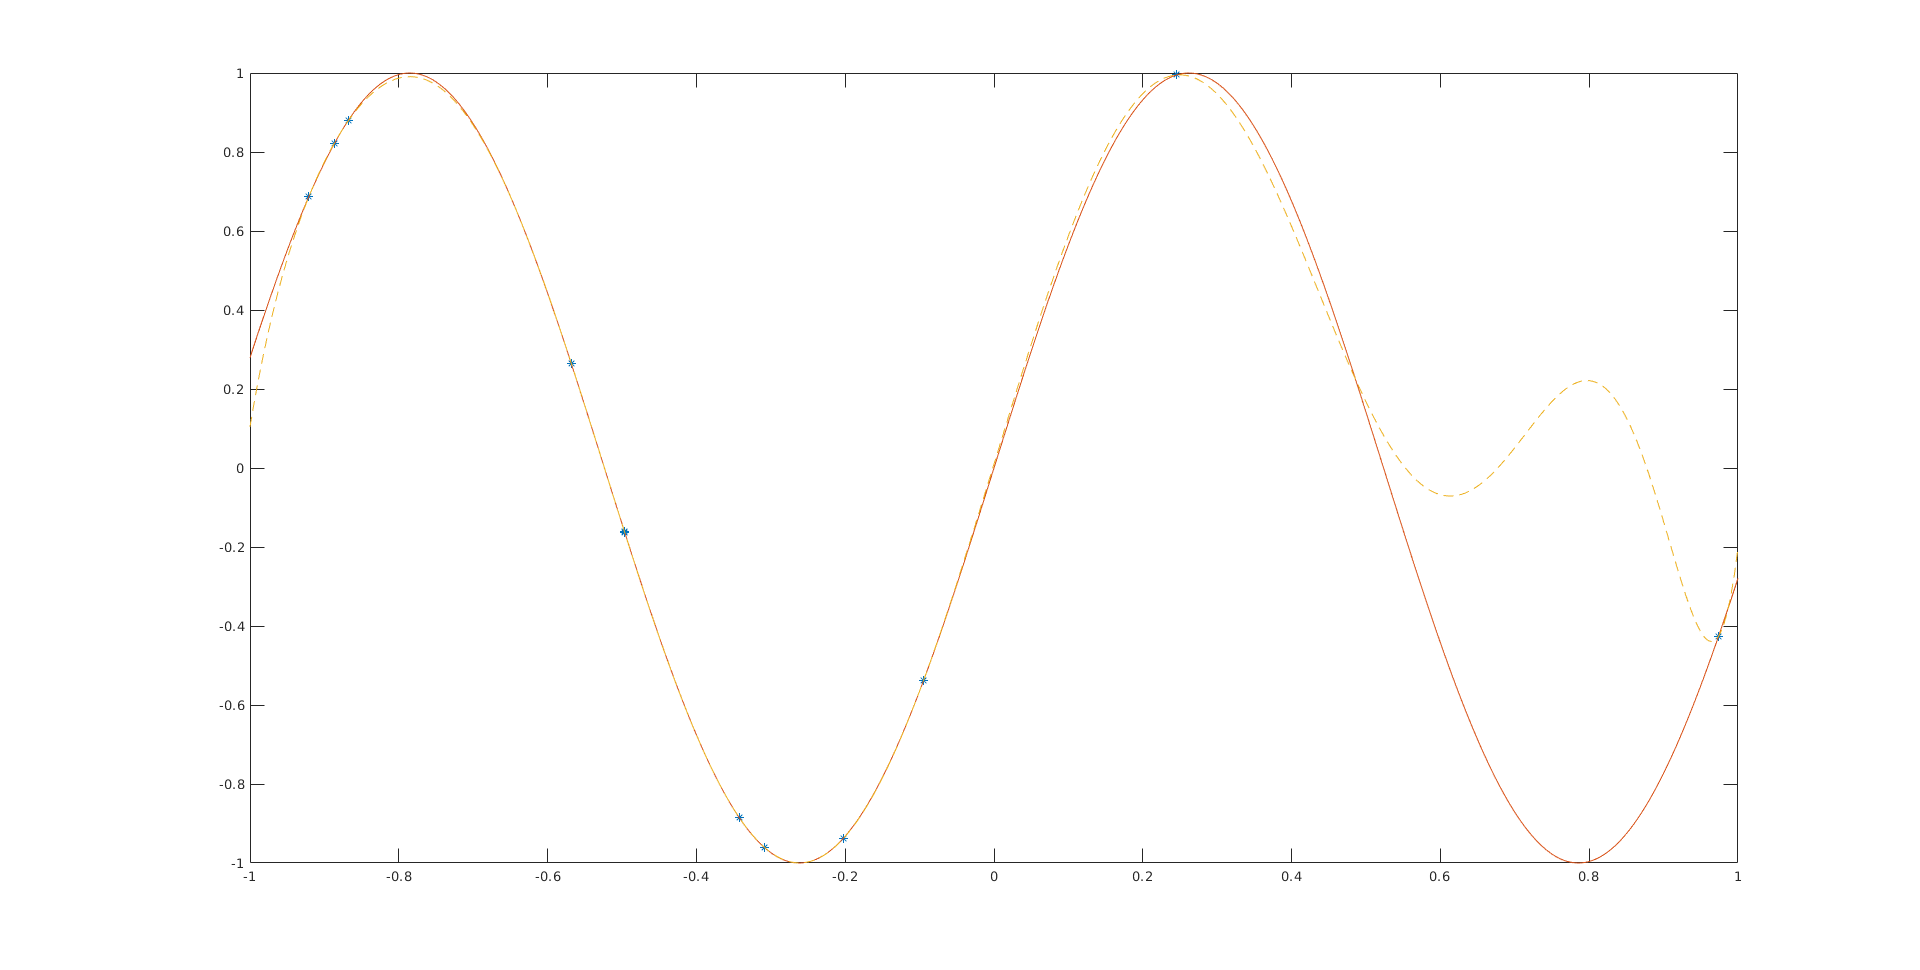
\includegraphics[scale=0.3]{figure/fig2.png}
\caption{using Tikhonov inverse}
\label{fig2}
\end{figure}

\begin{figure}[htbp]
\centering
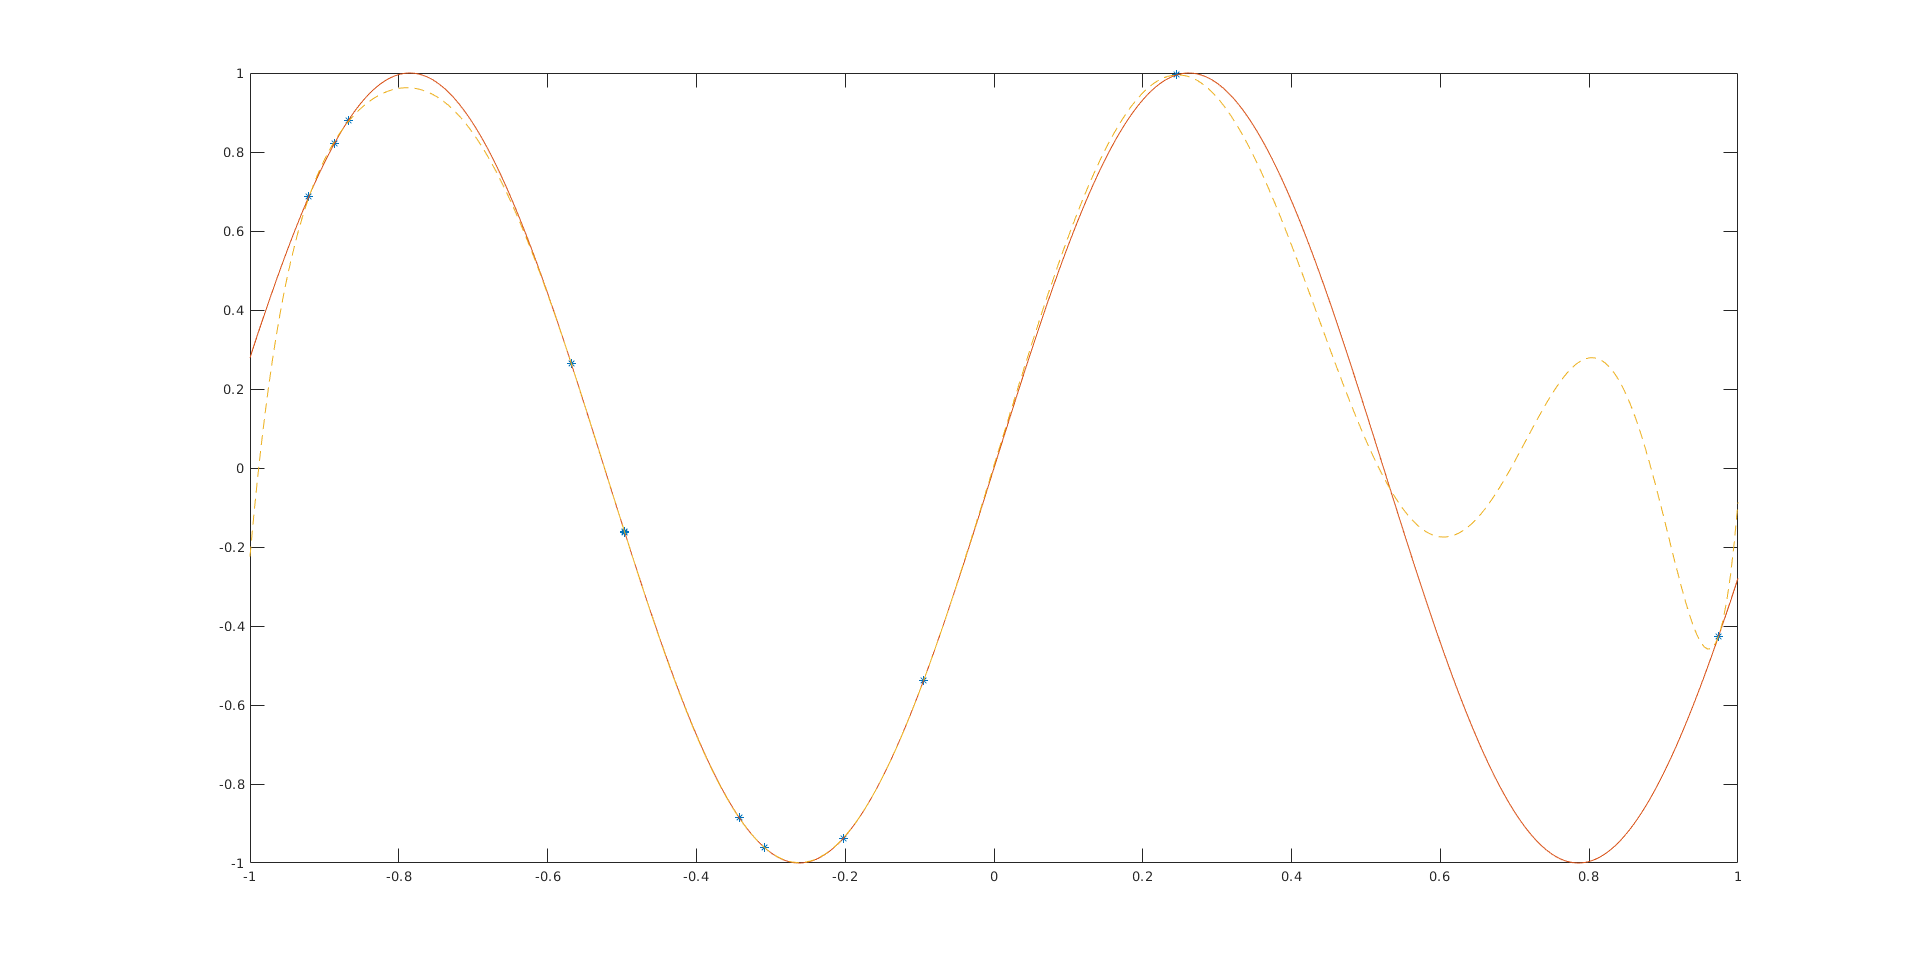
\includegraphics[scale=0.3]{figure/fig3.png}
\caption{using trucated SVD}
\label{fig3}
\end{figure}

\newpage 

\subsection*{Code}

\lstset{
	language=Octave,
	xleftmargin=3em,
}
\begin{lstlisting}
% Demonstration of overfitting in a polynomial regression problem.
% We approximate sin(6x) by sum c_j T_j(x) where T_j(x) are the
% Chebyshev polynomials, and determine the coefficients by a least
% squares fit with noise.

m = 12;      % Number of data points
n = 12;      % Number of expansion terms
sig = 1e-4;  % Noise level

% Set up interpolation and test points

x  = 2*rand(m,1)-1;
xt = linspace(-1,1,400)';

% Function values
fx  = sin(6*x);
fxt = sin(6*xt);
fxe = fx + sig*randn(m,1);

% Evaluate Chebyshev polynomials at points x and fit
A = chebmatrix(x, n);
c = A\fxe;

% Predict at test grid xt
At = chebmatrix(xt,n);
fxt_pred = At*c;

% Tikhonov inverse
[u z v] = svd(A, 'econ');
lambda = sqrt(z(1,1)) / 100;
d = (A'*A + lambda^2*eye(n,n)) \ (A' * fxe);

% truncated_SVD
threshold = 0.5
infinity = 1e7
% [u z v] = svd(A, 'econ');
for i=1:length(z)
	if z(i,i) < threshold
		z(i,i) = infinity;
	end
end
newA = u*z*v';
e = newA\fxe;

% Show the norm of the test error
test_err = fxt-fxt_pred;
fprintf('Test error: %e\n', norm(test_err));
fprintf('After using Tikhonov inverse, Test error: %e\n', norm(fxt-At*d));
fprintf('After using trucated_SVD, Test error: %e\n', norm(fxt-At*e));

% Plot data
figure(1); plot(x, fxe, '*', xt, fxt, '-', xt, At*c, '--');
figure(2); plot(x, fxe, '*', xt, fxt, '-', xt, At*d, '--');
figure(3); plot(x, fxe, '*', xt, fxt, '-', xt, At*e, '--');
figure(4); semilogy(x, abs(fxe-fx), '*', xt, abs(fxt-At*c));

\end{lstlisting}


\end{document}
